% This is part of Un soupçon de mathématique sans être agressif pour autant
% Copyright (c) 2012-2013
%   Laurent Claessens
% See the file fdl-1.3.txt for copying conditions.

Ce chapitre contient les choses tapées mais qui sont hors programmes.

%+++++++++++++++++++++++++++++++++++++++++++++++++++++++++++++++++++++++++++++++++++++++++++++++++++++++++++++++++++++++++++ 
\section{Statistique descriptive}
%+++++++++++++++++++++++++++++++++++++++++++++++++++++++++++++++++++++++++++++++++++++++++++++++++++++++++++++++++++++++++++

%--------------------------------------------------------------------------------------------------------------------------- 
\subsection{Activité : mois de naissance}
%---------------------------------------------------------------------------------------------------------------------------

Prendre les mois de naissance des élèves, en séparant les groupes.
\begin{enumerate}
    \item
        Quel groupe a la proportion de naissance en mars la plus grande ?
    \item
        En tout quelle est la proportion des naissances en avril ?
    \item 
        Est-ce qu'on peut voir l'effet comme quoi les mois de \( 31\) jours son plus longs ? 
        \begin{enumerate}
            \item
                Quelle est la proportion d'élèves nés dans un mois de \( 31\) jours ?
            \item
                Il y a \( 7\) mois de $31$ jours contre \( 5\) de moins. Donc le résultat est biaisé.
            \item
                Calculer la \emph{fréquence} des naissances en naissances par mois.
        \end{enumerate}
\end{enumerate}


\begin{example}
    Comment manipuler des chiffres et la perception des coefficients des épreuves du bac. en utilisant à tort et à travers la notion de moyenne ?\\
    \url{http://allken-bernard.org/pierre/weblog/?p=2386}
\end{example}



\begin{definition}
    Une \defe{population}{population} est un ensemble fini. Une \defe{série statistique}{série statistique} sur une population est une fonction qui à chaque élément (individu) de la population fait correspondre une valeur.

    L'\defe{effectif}{effectif} d'une valeur est le nombre d'individus correspondant à la valeur.

    La \defe{fréquence}{fréquence} d'une valeur est le rapport
    \begin{equation}
        f=\frac{ \text{effectif de la valeur} }{ \text{effectif total} }
    \end{equation}
    où par «effectif total» nous entendons la taille de la population totale.
\end{definition}

La \defe{moyenne}{moyenne} d'une suite de nombres \( x_1,\ldots, x_n\) est
\begin{equation}
    \bar x=\frac{1}{ n }\sum_{i=1}^nx_i=\frac{ \text{somme des \( x_i\)} }{\text{nombre de données}}.
\end{equation}

\begin{example}
    Soit la suite de nombres
    \begin{equation}
        1,7,0,3,9,0,1,3,1,0,2,5,6,9,1,1,3,2,4.
    \end{equation}
    Il y a \( 19\) nombres. La moyenne est donnée par la fraction
    \begin{equation}
        \bar x=\frac{ 1+7+0+3+9+\ldots+3+2+4 }{ 19 }=\frac{ 58 }{ 19 }.
    \end{equation}

Python permet d'obtenir assez facilement une approximation numérique :
    \begin{verbatim}
>>> import numpy
>>> nombres=[1,7,0,3,9,0,1,3,1,0,2,5,6,9,1,1,3,2,4]
>>> numpy.mean(nombres)          # 'mean' signifie 'moyenne' en anglais.
3.0526315789473686 
    \end{verbatim}
\end{example}


%+++++++++++++++++++++++++++++++++++++++++++++++++++++++++++++++++++++++++++++++++++++++++++++++++++++++++++++++++++++++++++
\section{Dessiner en vraie grandeur}
%+++++++++++++++++++++++++++++++++++++++++++++++++++++++++++++++++++++++++++++++++++++++++++++++++++++++++++++++++++++++++++

La perspective cavalière n'est pas parfaite; aucune perspective n'est parfaite. Étant donné que les surfaces sont déformées, nous voudrions être capables de dessiner certaines surfaces sans déformations. C'est ce que nous appelons \emph{dessiner en vraie grandeur}.

\begin{Aretenir}
    Lorsqu'on demande de dessiner une surface en vraie grandeur, voici les mouvements «de base» que vous êtes autorisés à effectuer \emph{dans un plan}.
    \begin{enumerate}
        \item
            Tracer des segments de longueur \emph{entières} !
        \item
            Tracer des cercles dont le centre et un point sont donnés.
        \item
            Tracer les droites dont deux points sont donnés.
        \item
            Considérer les intersections des droites et cercles.
    \end{enumerate}
    À partir ce ces mouvements, il est possible de tracer de nombreuses choses, dont par exemple
    \begin{enumerate}
        \item
            Le milieu du segment \( [AB]\) lorsque les points \( A\) et \( B\) sont donnés.
        \item
            Si la droite \( d\) et le point \( I\) plan sont donnés, la perpendiculaire à \( d\) passant par \( I\).
        \item
            Si les points \( d\) du plan et le point \( I\) sont donnés, la parallèle à \( d\) passant par \( I\).
    \end{enumerate}
\end{Aretenir}

\begin{proof}
    Nous allons donner les constructions.
    \begin{enumerate}
        \item
            Soient \( A\) et \( B\) données. À construire : la médiatrice du segment \( [AB]\). Avec cela, nous connaîtrons le milieu. Le technique est simple : il suffit de tracer deux cercles de même rayons \( r\) centrés en \( A\) et en \( B\). Les points d'intersection \( I\) et \( J\) donnent la médiatrice. En effet, par construction \( I\) est équidistant de \( A\) et \( B\) parce que \( I\) est à la fois sur le cercle de rayon \( r\) autour de \( A\) et sur le cercle de rayon \( r\) autour de \( B\). Or nous savons que les points équidistants de \( A\) et \( B\) sont sur la médiatrice du segment \( [AB]\).

            Pour la même raison, le point \( J\) est également sur la médiatrice. Cela fait que \( (IJ)\) coupe \( [AB]\) en son milieu.

Cette construction est illustrée sur la figure \ref{LabelFigIsoceleVdviOE}. % From file IsoceleVdviOE
\newcommand{\CaptionFigIsoceleVdviOE}{Le triangle \( AJB\) est isocèle.}
\input{Fig_IsoceleVdviOE.pstricks}

        \item

            Soient donnés la droite \( d\) et le point \( I\). Nous construisons un cercle centré en \( I\) et nous nommons \( A\) et $B$ les points d'intersection entre ce cercle et la droite \( A\). Par construction le triangle \( AIB\) est isocèle. Donc \( I\) est sur la médiatrice du segment \( [AB]\). La construction précédente permet de construire cette médiatrice qui sera alors perpendiculaire à \( d\) passant par \( I\).

Un dessin de la situation est proposé à la figure \ref{LabelFigPerpSegqrbMBZ}. % From file PerpSegqrbMBZ
\newcommand{\CaptionFigPerpSegqrbMBZ}{Le triangle \( AIB\) est isocèle et la droite rouge est la médiatrice de \( [AB]\).}
\input{Fig_PerpSegqrbMBZ.pstricks}

    \item
        
        Si la droite \( d\) et le point \( I\) sont donnés, pour construire la parallèle à \( d\) passant par \( I\), il suffit de construire la perpendiculaire \( d'\) à \( d\) passant par \( I\) et ensuite la perpendiculaire à \( d'\) passant par \( I\).

    \end{enumerate}
\end{proof}


Quelque dessin qui ne sont plus utilisés :


Des exemples sont donnés à la figure \ref{LabelFigPositionsDroitesbnYIsH}. % From file PositionsDroitesbnYIsH
\newcommand{\CaptionFigPositionsDroitesbnYIsH}{Droites coplanaires ou non.}
\input{Fig_PositionsDroitesbnYIsH.pstricks}

%See also the subfigure \ref{LabelFigPositionsDroitesbnYIsHssLabelSubFigPositionsDroitesbnYIsH0}
%See also the subfigure \ref{LabelFigPositionsDroitesbnYIsHssLabelSubFigPositionsDroitesbnYIsH1}
%See also the subfigure \ref{LabelFigPositionsDroitesbnYIsHssLabelSubFigPositionsDroitesbnYIsH2}
Notez en particulier la figure \ref{LabelFigPositionsDroitesbnYIsHssLabelSubFigPositionsDroitesbnYIsH3} sur laquelle les droites \( (FH)\) et \( (AC)\) ne sont pas sécantes !


%+++++++++++++++++++++++++++++++++++++++++++++++++++++++++++++++++++++++++++++++++++++++++++++++++++++++++++++++++++++++++++ 
\section{Surfaces dans un cube}
%+++++++++++++++++++++++++++++++++++++++++++++++++++++++++++++++++++++++++++++++++++++++++++++++++++++++++++++++++++++++++++

La figure \ref{LabelFigDesSections} montre un cube. Êtes-vous capables de donner la nature des surfaces coloriées ?
\newcommand{\CaptionFigDesSections}{Exercice de vision dans l'espace.}
\input{Fig_DesSections.pstricks}
Le triangle vert est isocèle et rectangle parce que deux de ses côtés sont des arrêtes du cube. Le triangle rouge est plus troublant, mais il est équilatéral : ses trois côtés sont des diagonales des faces du cube. Notez que \emph{sur le dessin}, les trois côtés ont des longueur différentes.

%+++++++++++++++++++++++++++++++++++++++++++++++++++++++++++++++++++++++++++++++++++++++++++++++++++++++++++++++++++++++++++
\section{Les règles de la perspective cavalière}
%+++++++++++++++++++++++++++++++++++++++++++++++++++++++++++++++++++++++++++++++++++++++++++++++++++++++++++++++++++++++++++

Lorsque nous dessinons en trois dimension, nous prenons les conventions suivantes qui définissent la \defe{\wikipedia{fr}{Perspective_cavalière}{perspective cavalière}}{perspective!cavalière}.

\begin{Aretenir}
    D'abord nous choisissons
    \begin{enumerate}
        \item
            Nous choisissons un \defe{angle de fuite}{angle!de fuite} \( \alpha\) qui sera entre \unit{30}{\degree} et \( \unit{45}{\degree}\) avec l'horizontale\footnote{Sur une feuille à carreaux, le plus simple est de prendre \unit{45}{\degree}.}.
        \item
            Un \defe{coefficient de réduction}{coefficient de réduction} que nous noterons \( k\) et qui sera compris entre \( 0\) et \( 1\).
    \end{enumerate}

    Ensuite nous prenons les correspondances suivantes entre la réalité et le dessin :
    \begin{center}
        \begin{tabular}{|p{7.5cm}|p{7.5cm}|}
            \hline
            {\bf dans la réalité}&{\bf sur le dessin}\\
            \hline\hline
            Segment caché  & Segment pointillé\\
            \hline
            Segment parallèle à la feuille de dessin & Segment représenté en vraie grandeur\\
            \hline
            Segment perpendiculaire à la feuille de dessin & Segment faisant un angle \( \alpha\) avec l'horizontale.\\
            \hline
            Une arrête de longueur \( l\) perpendiculaire à la feuille de dessin & Une arrête de longueur \( k\times l\) faisant un angle \( \alpha\) avec l'horizontale.\\
            \hline
        \end{tabular}
    \end{center}
\end{Aretenir}

\begin{minipage}{0.485\textwidth}
    Un carré fait un demi-centimètre. 
    \begin{itemize}
        \item Quel est l'angle de fuite utilisé ?
        \item Quel est le coefficient de réduction utilisé ?
    \end{itemize}
\end{minipage}
\hspace{1mm}
\begin{minipage}{0.6\textwidth}
    \center
    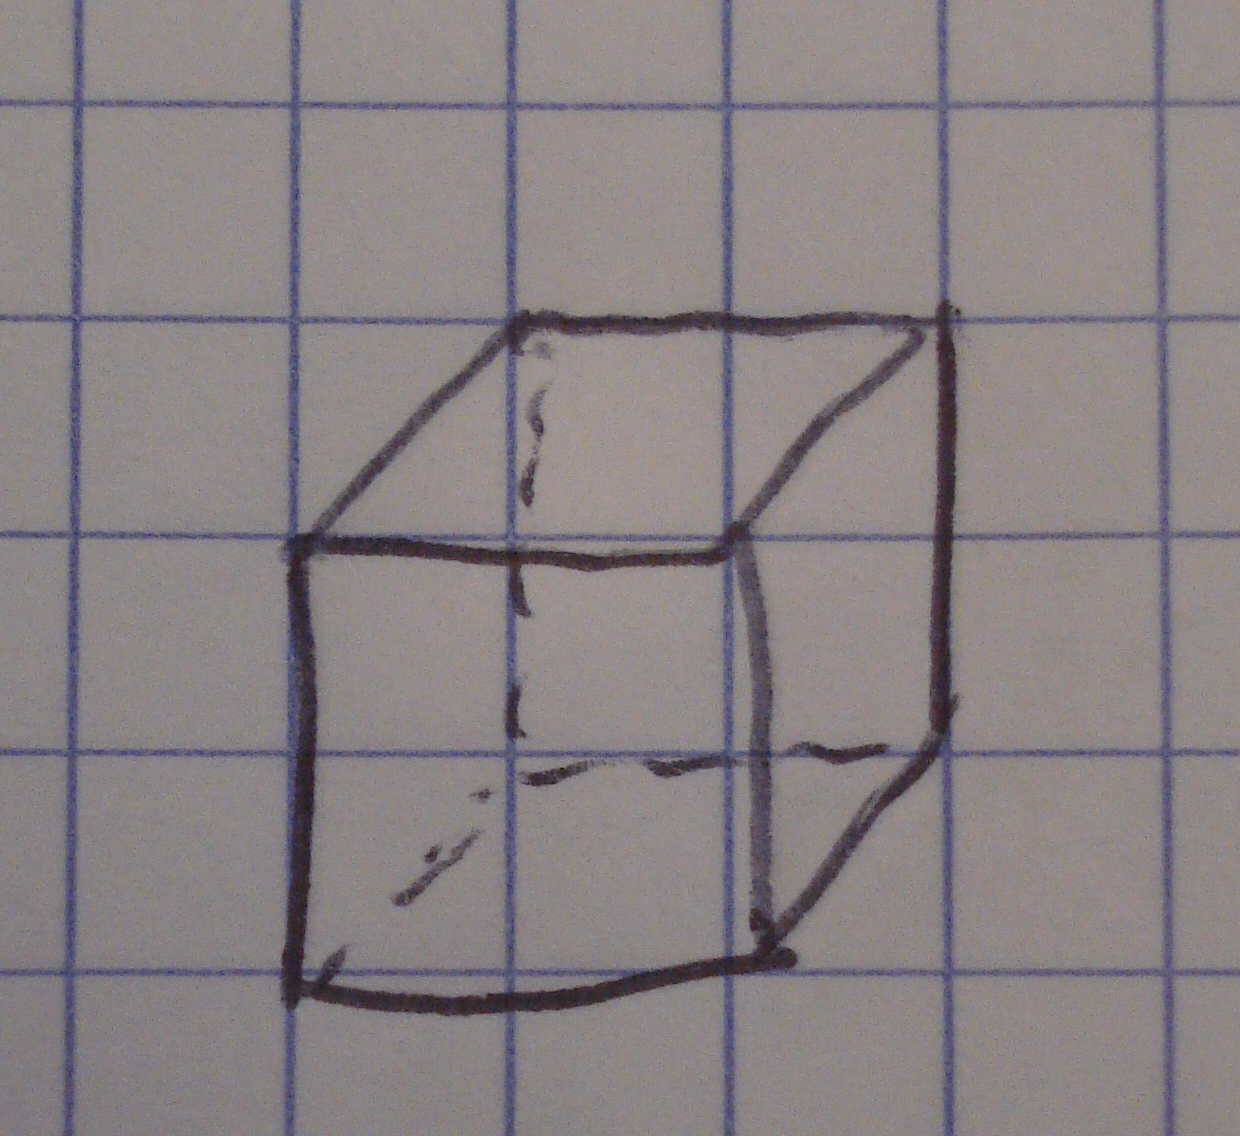
\includegraphics[width=0.6\textwidth]{cube_quadrill.png}
\end{minipage}

\begin{propriete}
    La perspective cavalière respecte les conditions suivantes.
    \begin{enumerate}
        \item
             Deux segments parallèles dans la réalité sont représentés par deux segments parallèles sur le dessin.
         \item
             Trois points alignés dans la réalité sont représentés par trois points alignés sur le dessin.
         \item
             Si \( M\) est le milieu du segment \( [AB]\) dans la réalité, alors \( M\) est le milieu du segment \( [AB]\) dans la réalité.
         \item
             La perspective cavalière respecte les proportions. C'est à dire que si le segment \( [AB]\) est \( p\) fois plus grand que le segment \( [CD]\) dans la réalité, alors il sera \( p\) fois plus grand sur le dessin.
    \end{enumerate}
\end{propriete}

Le cube de la figure \ref{LabelFigCubeLFZuiW} est dessiné avec \( \alpha=\unit{45}{\degree}\) et \( k=0.5\). Notez que les côtés parallèles restent parallèles.
\newcommand{\CaptionFigCubeLFZuiW}{Les segments perpendiculaires à la feuille sont de longueur moitié des autres.}
\input{Fig_CubeLFZuiW.pstricks}

La perspective cavalière n'est pas parfaite; il est aisé de créer des illusions d'optique comme celle de la figure \ref{LabelFigIllusionNHwEtp}. % From file IllusionNHwEtp
\newcommand{\CaptionFigIllusionNHwEtp}{Une petite illusion d'optique facile.}
\input{Fig_IllusionNHwEtp.pstricks}

%+++++++++++++++++++++++++++++++++++++++++++++++++++++++++++++++++++++++++++++++++++++++++++++++++++++++++++++++++++++++++++ 
\section{Exercices}
%+++++++++++++++++++++++++++++++++++++++++++++++++++++++++++++++++++++++++++++++++++++++++++++++++++++++++++++++++++++++++++

\Exo{Seconde-0096}
\Exo{Seconde-0097}

%+++++++++++++++++++++++++++++++++++++++++++++++++++++++++++++++++++++++++++++++++++++++++++++++++++++++++++++++++++++++++++ 
\section{AP sur les problèmes climatiques et de pétrole}
%+++++++++++++++++++++++++++++++++++++++++++++++++++++++++++++++++++++++++++++++++++++++++++++++++++++++++++++++++++++++++++

Je voudrais faire une AP basée sur la vidéo de Jean-Marc Jancovici à l'ENS :
\url{http://savoirsenmultimedia.ens.fr/expose.php?id=572}

Montrer ça à des élèves de seconde est le super-défi :)



%+++++++++++++++++++++++++++++++++++++++++++++++++++++++++++++++++++++++++++++++++++++++++++++++++++++++++++++++++++++++++++
\section{Regardons des graphiques}
%+++++++++++++++++++++++++++++++++++++++++++++++++++++++++++++++++++++++++++++++++++++++++++++++++++++++++++++++++++++++++++

Les graphiques sont souvent tirés de wikipédia. Si vous voulez plus d'informations, lisez \url{http://www.manicore.com/}, ou bien regardez le cours \href{http://www.mines-paristech.fr/ingenieurcivil/SitesIC/Balado/Climat_som.html}{en ligne}, en particulier la deuxième heure du troisième cours donne les facteurs d'émissions dans le monde et en France.

%---------------------------------------------------------------------------------------------------------------------------
\subsection{Émissions par secteurs}
%---------------------------------------------------------------------------------------------------------------------------

\EpsOrPdfincludegraphics[width=17cm]{Emission_de_GES}
Graphique en provenance de l'article \wikipedia{fr}{Gaz_à_effet_de_serre}{gaz à effet de serre} de wikipédia.

\begin{enumerate}
    \item
        Quel est le secteur qui émets le plus ?
    \item
        Est-ce que l'agriculture émet beaucoup de dioxyde de carbone ?
    \item
        À partir des deux graphiques du bas, est-ce que vous êtes capables de retrouver le \( 12.5\%\) de l'agriculture donnés dans le graphique du haut ?
\end{enumerate}

%---------------------------------------------------------------------------------------------------------------------------
\subsection{Découvertes de pétrole}
%---------------------------------------------------------------------------------------------------------------------------

Regardons un instant le graphique suivant, provenant de l'article \wikipedia{fr}{Pic_pétrolier}{Pic pétrolier} de wikipédia.

\EpsOrPdfincludegraphics[width=17cm]{Decouvertes-petrole}

\begin{enumerate}
    \item
        Quelle est l'année où on a découvert le plus de pétrole ?
    \item
        Quelle est l'année où on a consommé le plus de pétrole ?
    \item
        En quelles années on a consommé autant qu'on a découvert ?
    \item
        Que pensez-vous de l'affirmation «ce qui reste comme réserve est la surface jaune au-dessus de la ligne rouge» ?
\end{enumerate}
Pour aller plus loin, remarquer la cassure assez nette de la croissance de la production vers 1975. Juste par curiosité, faites quelque recherches sur l'histoire de la croissance économique, de la dette publique et le chômage en France (et en Europe). Est-ce que les années 1970 ont été spéciales de ce point de vue ?

%---------------------------------------------------------------------------------------------------------------------------
\subsection{Températures}
%---------------------------------------------------------------------------------------------------------------------------

\EpsOrPdfincludegraphics[width=17cm]{Instrumental_Temperature_Record_fr}
Graphique en provenance de l'article \wikipedia{fr}{Réchauffement_climatique}{réchauffement climatique} de wikipédia.

Le zéro de ce graphique est la moyenne 1961-1990.

\begin{enumerate}
    \item
        Quelle est la dernière année «normale» ?
    \item
        Quelle est l'année la plus chaude ?
    \item
        Quelle est l'année la plus froide ?
\end{enumerate}

%---------------------------------------------------------------------------------------------------------------------------
\subsection{Consommation de pétrole}
%---------------------------------------------------------------------------------------------------------------------------

Lire le tableau suivant :
\begin{center}
\begin{tabular}[h]{|c|c|c|c|c|c|c|c|c|}
année&
2001&
2002&
2003&
2004&
2005&
2006&
2007&
2008\\
consommation (Mb/j)&
76,8&
77,7&
79,1&
81,8&
83,1&
83,8&
84,9&
84,5
\end{tabular}
\end{center}

Calculer le pourcentage d'augmentation année par année. Que s'est-il passé en 2008 ?


%---------------------------------------------------------------------------------------------------------------------------
\subsection{Orthogonalité}
%---------------------------------------------------------------------------------------------------------------------------

% Note : l'orthogonalité n'a pas l'air d'être au programme de seconde.
\Exo{smath-0077}
\Exo{smath-0082}



%+++++++++++++++++++++++++++++++++++++++++++++++++++++++++++++++++++++++++++++++++++++++++++++++++++++++++++++++++++++++++++ 
\section{Intervalle de fluctuation}
%+++++++++++++++++++++++++++++++++++++++++++++++++++++++++++++++++++++++++++++++++++++++++++++++++++++++++++++++++++++++++++

Pour reprendre le cas de l'acné, nous considérons la population française totale (65 millions de personnes), et nous voulons savoir si les \emph{jelly bean} sont liés à l'acné.

Il n'est évidemment pas question de tester toute la France. L'étude est en plusieurs étapes.
\begin{enumerate}
    \item
        On va demander aux spécialistes quel est le pourcentage de français souffrant d'acné. Disons pour l'exemple que le résultat soit de \( 20\%\).
    \item
        On prend un échantillon de français (disons \( 1000\)) mangeant régulièrement des \emph{jelly beans}, et on compte combien ont de l'acné.
    \item
        Si plus de \( 20\%\) des personnes de l'échantillon présente de l'acné, alors on se pose des questions.
\end{enumerate}

Dans l'échantillon, nous nous attendons à avoir 
\begin{equation}
    \frac{ 20 }{ 100 }\times 1000=200
\end{equation}
personnes développant de l'acné si les \emph{jelly beans} ne sont pas liées à l'acné. 

Évidemment, si on en a \( 201\) ou \( 199\), ce n'est pas un problème. La question précise à laquelle nous devons répondre est :
\begin{quote}
    À partir de combien de personnes développant de l'acné, pouvons-nous dire que ça ne peut pas être le fruit du hasard ?
\end{quote}
Et c'est la réponse à cette questions que ne connaît manifestement pas le journaliste qui a écrit l'article en fin de blague.


Comment cela s'applique à notre étude de \emph{jelly bean} ? 
\begin{description}
    \item[Résumé des données]
        La proportion des français présentant de l'acné est dite de \( p=0.2\), et nous avons prélevé un échantillon de taille \( n=1000\). 
    \item[Intervalle de fluctuation] 
        Donc dans notre échantillon nous avons \( 95\%\) de chances que la fréquence soit dans l'intervalle
        \begin{equation}
            \mathopen[ 0.2-\frac{1}{ \sqrt{1000} } ; 0.2+\frac{1}{ \sqrt{1000} } \mathclose]\simeq\mathopen[ 0.168 ; 0.231 \mathclose]
        \end{equation}
        parce que \( \frac{1}{ \sqrt{1000} }\simeq 0.03162\).
    \item[Transformation en effectifs]

        Une fréquence de \( 0.168\) dans un échantillon de \( 1000\) individus revient à \( 168\) individus et une fréquence de \( 0.231\) revient à \( 231\) individus.

        Nous avons donc \( 95\%\) de chances que, en faisant l'étude sur \( 1000\) personnes, le nombre de personnes présentant de l'acné soit compris ente \( 168\) et \( 231\).
    \item[Décider si les \emph{jelly bean} provoquent l'acné]
        Si sur un échantillon de \( 1000\) personnes mangeant des \emph{jelly bean} nous en avons par exemple \( 260\) qui présentent de l'acné, alors nous pouvons dire que les \emph{jelly bean} sont liés à l'acné au sens où il y a moins de \( 5\%\) de chances que le résultats puisse s'expliquer par le hasard.

        Si sur cet échantillon de \( 1000\) personnes, nous en avons \( 180\), nous ne dirons rien. Avoir \( 180\) personnes avec de l'acné dans un échantillon de \( 1000\) personnes est «raisonnable» par rapport à la moyenne nationale.
\end{description}

\begin{remark}
    Dans le cas où le nombre de personnes présentant de l'acné dépasse les \( 231\), ça ne veut pas dire que les \emph{jelly bean} \emph{provoquent} l'acné. Cela veut juste dire qu'elles sont \emph{corrélées} à l'acné, et qu'il y a même \( 5\%\) de chances que ce soit un pur hasard.
\end{remark}


%+++++++++++++++++++++++++++++++++++++++++++++++++++++++++++++++++++++++++++++++++++++++++++++++++++++++++++++++++++++++++++ 
\section{Intervalle de confiance}
%+++++++++++++++++++++++++++++++++++++++++++++++++++++++++++++++++++++++++++++++++++++++++++++++++++++++++++++++++++++++++++

Nous avons vu l'intervalle de fluctuation. Il s'agit, lorsqu'on connaît la proportion \( p\) des individus présentant un certain caractère dans la population globale, de savoir si la fréquence $f$ observée dans un échantillon de taille \( n\) est crédible ou pas.

Ici nous allons poser la question inverse. Nous ne connaissons pas la proportion dans la population globale, mais seulement une fréquence dans un échantillon.

Soit donc une population dont une proportion inconnue \( p\) présente un caractère. Nous en tirons un échantillon de taille \( n\), et nous mesurons la fréquence \( f\) d'apparition du caractère dans cet échantillon.

Question : sachant \( f\), que peut-on dire de \( p\) ? 

Ce que nous savons, c'est qu'il y a \( 95\%\) de chances que 
\begin{equation}
    f\in\mathopen[ p-\frac{1}{ \sqrt{n}} , 1+\frac{1}{ \sqrt{n} } \mathclose].
\end{equation}
Cet intervalle peut être décortiqué de la façon suivante :
\begin{equation}
\xymatrix{%
    &   f\in\mathopen[ p-\frac{1}{ \sqrt{n}} , p+\frac{1}{ \sqrt{n} } \mathclose]\ar[rd]\ar[ld] &  \\
    f\geq p-\frac{1}{ \sqrt{n}}\ar[d]&&f\leq p+\frac{1}{ \sqrt{n}}  \ar[d]\\
    p\leq f+\frac{1}{ \sqrt{n}}\ar[rd] && f-\frac{1}{ \sqrt{n}}\leq p\ar[ld]\\
    & p\in\mathopen[ f-\frac{1}{ \sqrt{n} } , f+\frac{1}{ \sqrt{n}} \mathclose]  &
   }
\end{equation}

\begin{center}

           \ifpdf
            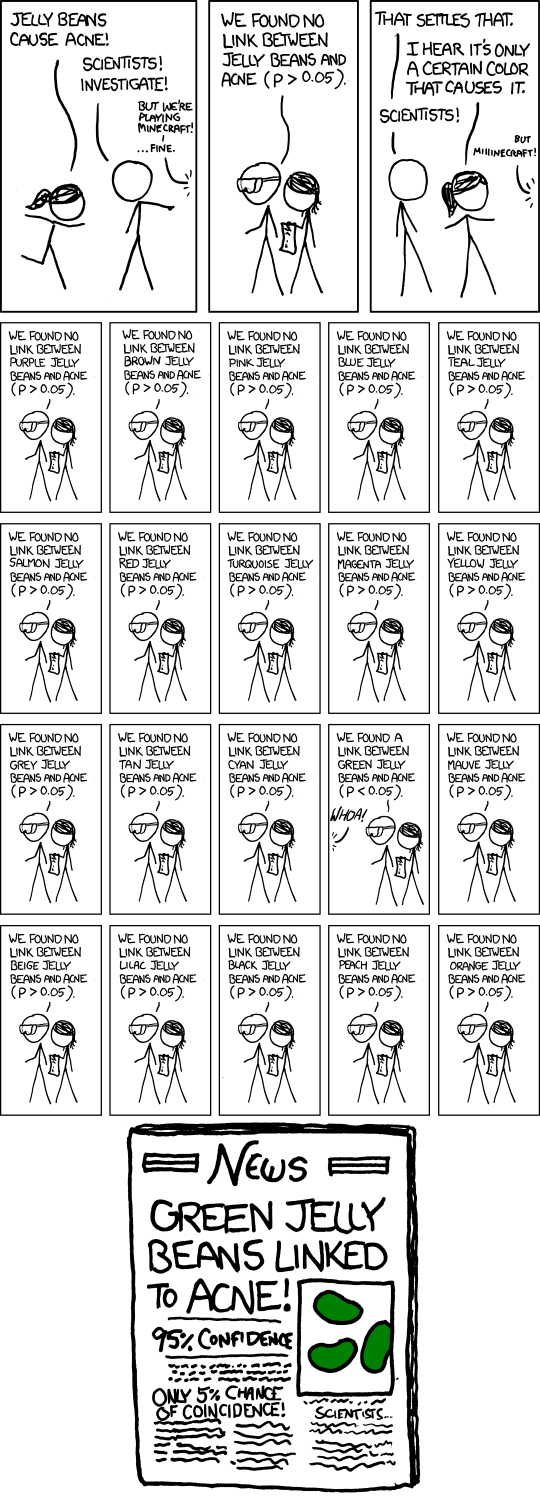
\includegraphics[width=8cm]{significant.png}
        \else
            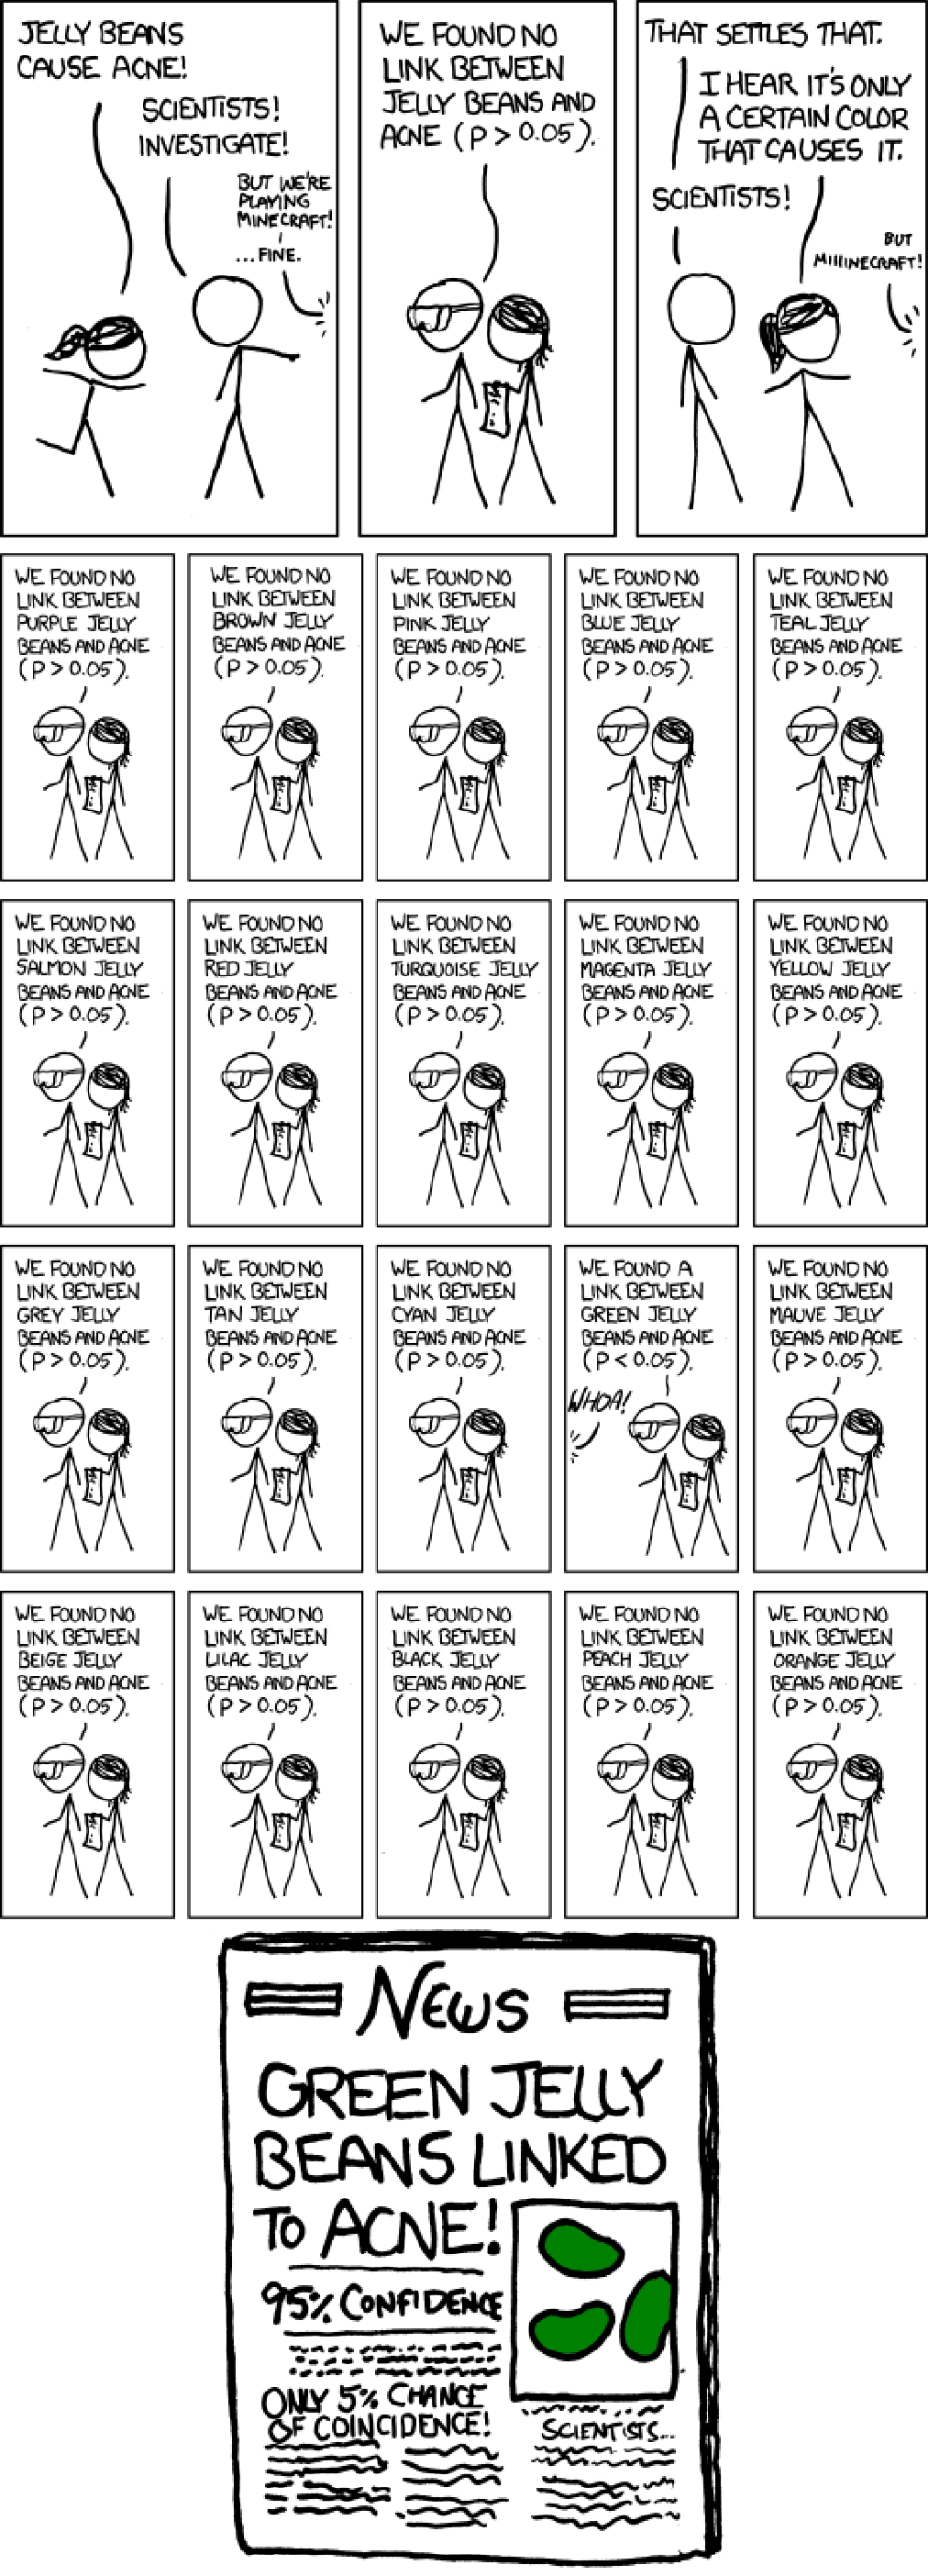
\includegraphics[width=8cm]{significant.eps}

            \fi

            \url{http://xkcd.com/882/}, image publiée sous licence \href{http://xkcd.com/license.html}{CreativeCommons}.

\end{center}


